\documentclass[11pt,a4paper]{article}
\usepackage[margin=22mm]{geometry}
\usepackage[T1]{fontenc}
\usepackage{lmodern,amsmath,amssymb,booktabs,array,tikz,listings,enumitem}
\usepackage[hidelinks]{hyperref}
\usetikzlibrary{arrows.meta}
\lstset{basicstyle=\ttfamily\small,breaklines=true,columns=fullflexible,frame=single}
\setlength{\parindent}{0pt}
\setlength{\parskip}{6pt}
\title{Digital System Design and Implementation\\Final Exam (113/06/04)\\Spring 2024}
\author{Question transcription}
\date{}
\begin{document}
\maketitle
\textbf{Total points: 100.}

\textit{Source: \texttt{FinalExam.pdf}, four pages. Text is transcribed below; the essential contents of the figures are redrawn as editable tables and diagrams. The original PDF is retained separately. The original HDL template DSD.v was not supplied with this PDF. Editorial notes are marked explicitly.}

\textbf{Original examination instructions}
\begin{itemize}[nosep]
\item Please download the template file DSD.v, which contains all the required I/O in each question and rename it as DSDxxxxxxxxx.v or DSDxxxxxxxxx.sv, where x is your student ID, for example, DSD107501001.v.
\item Use the template to ensure your module and input as well as output ports having the same module/port names as described in the following.
\item Discussion is not allowed, but you can check your own lecture notes.
\item If partial function is correct, you can still get some points. So, try to write codes that can work even that only partial functions are implemented.
\end{itemize}

In this final exam, we want to process one-dimensional sequence in a given pattern. Please write each module first. The clock signal is called ``Clock'' and the asynchronous active-high reset signal, called ``Reset'', is used for all the questions.

\section*{1. Decrementer (10\%)}
Please write a 5-bit decrementer which can count down after reset. Its timing diagram is given as follows. Its output signal is called ``DecOut''.
\par\medskip\noindent\begin{minipage}{\linewidth}
\begin{lstlisting}
module Decrementer(DecOut, Clock, Reset);
endmodule
\end{lstlisting}
\end{minipage}\par
\begin{center}
\begin{tabular}{lrrrrrrrr}
\toprule
Figure 1 output & \multicolumn{8}{c}{Successive values after reset}\\
\midrule
DecOut & 0 & 31 & 30 & 29 & $\cdots$ & 1 & 0 & 31\\
\bottomrule
\end{tabular}
\end{center}
\textit{Figure 1: Timing diagram of a decrementer. Reset is initially asserted; counting occurs at the rising edges of Clock.}

\section*{2. Incrementer/decrementer with enable (16\%)}
Now, extend the function of the module in Q1. We want to construct a module that can be an incrementer or decrementer according to the control signal ``IorD'' shown in Fig.~2. Hence, it can generate the output by addition or subtraction. In addition, one input signal, called ``Enable'', is used to control the operation of the module. If it is low, then the module will keep its state.
\par\medskip\noindent\begin{minipage}{\linewidth}
\begin{lstlisting}
module Counting(CountOut, IorD, Enable, Clock, Reset);
endmodule
\end{lstlisting}
\end{minipage}\par
\begin{center}
\begin{tabular}{lp{105mm}}
\toprule
Figure 2 signal & Content of the original timing diagram\\
\midrule
Reset & Initially high, then low.\\
IorD & High during incrementing; low during decrementing.\\
Enable & Low during the two hold intervals.\\
CountOut & $0,0,1,2,3,3,4,\ldots,28,29,28,27,27,27,26,\ldots$\\
\bottomrule
\end{tabular}
\end{center}
\textit{Figure 2: Timing diagram of the counting module.}

\section*{3. Generate the up/down control pattern (16\%)}
We want to generate a special pattern for accessing the elements of a matrix that is stored in a memory array. Because the matrix is block diagonal, which means that the non-zero elements exist along the diagonal and in a square shape as shown in Fig.~3(a), we need to generate the special sequence as shown in Fig.~3(a) to control the module ``Counting'' in Q2. Assume that the size of the block along the diagonal is $3\times3$. You need to generate a signal, called ``UpDown'', as shown in Fig.~3(b), where ``Start'' signal triggers the operation.
\par\medskip\noindent\begin{minipage}{\linewidth}
\begin{lstlisting}
module GenerateUpDownCtr(UpDown, Start, Clock, Reset);
endmodule
\end{lstlisting}
\end{minipage}\par
\begin{center}
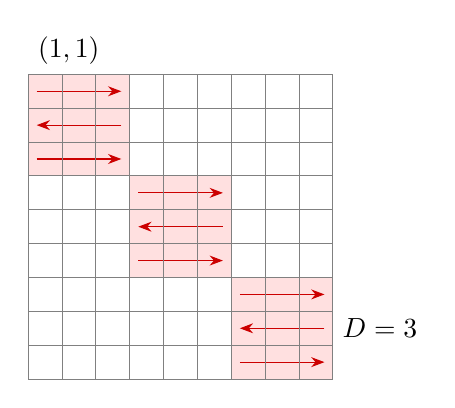
\begin{tikzpicture}[x=0.43cm,y=0.43cm]
\foreach \b in {0,3,6} {
  \fill[red!12] (\b,-\b) rectangle (\b+3,-\b-3);
  \draw[red!80!black,-{Stealth}] (\b+.25,-\b-.5) -- (\b+2.75,-\b-.5);
  \draw[red!80!black,-{Stealth}] (\b+2.75,-\b-1.5) -- (\b+.25,-\b-1.5);
  \draw[red!80!black,-{Stealth}] (\b+.25,-\b-2.5) -- (\b+2.75,-\b-2.5);
}
\draw[step=1,gray] (0,0) grid (9,-9);
\node[anchor=south west] at (0,0) {$(1,1)$};
\node[anchor=west] at (9,-7.5) {$D=3$};
\end{tikzpicture}
\qquad
\begin{tabular}{crrrr}
\toprule
Row & 1 & 2 & 3 & 4\\
\midrule
Clock cycles & 3 & 3 & 3 & 3\\
UpDown & 1 & 0 & 1 & 1\\
\bottomrule
\end{tabular}
\end{center}
\textit{Figure 3: (a) Access pattern in a block-diagonal matrix. Rows are scanned right, left, right within each block, then the next diagonal block starts. (b) After Start, UpDown is high for row~1, low for row~2, and high for rows~3 and~4; each row lasts three clock cycles. The three-row pattern repeats in subsequent blocks. Start is drawn low before operation and high thereafter.}

\section*{4. Generate row and column indices (24\%)}
Now, we want to generate the row index and column index, counting from 1, to access the elements of the matrix according to the setting of D. Assume that the matrix size along the row or the column is smaller than 64. Hence, 6 bits are reserved for output signals ``RIndx'' and ``CIndx'', corresponding to row index and column index. Note that you need to call module ``Counting'' in Q2 and ``GenerateUpDownCtr'' in Q3. Similarly, ``Start'' signal triggers the operation. The signal ``NewBlock'' asserts when the first element in the diagonal block appears. (We will replace the correct one when testing. So, don't worry about the correctness of your codes in Q2 and Q3. Just focus on this question given the correct modules in Q2 and Q3.) The timing diagram of the input and output signals is shown in Fig.~4.
\par\medskip\noindent\begin{minipage}{\linewidth}
\begin{lstlisting}
module GenerateRCIndex(NewBlock, RIndx, CIndx, Start, Clock, Reset);
Counting UQ2(.CountOut(), .IorD(), .Enable(), .Clock(), .Reset());
GenerateUpDownCtr UQ3(.UpDown(), .Start(), .Clock(), .Reset());
endmodule
\end{lstlisting}
\end{minipage}\par
\begin{center}
\small
\begin{tabular}{lrrrrrrrrrrrr}
\toprule
Row in Fig. 4 & \multicolumn{3}{c}{1} & \multicolumn{3}{c}{2} & \multicolumn{3}{c}{3} & \multicolumn{3}{c}{4}\\
\midrule
RIndx & 1&1&1&2&2&2&3&3&3&4&4&4\\
CIndx & 1&2&3&3&2&1&1&2&3&4&5&6\\
NewBlock & 1&0&0&0&0&0&0&0&0&1&0&0\\
\bottomrule
\end{tabular}
\end{center}
\textit{Figure 4: Before Start, both indices and NewBlock are zero. Each column of this table denotes one output interval between consecutive rising clock edges.}

\section*{5. Two-port register file (16\%)}
Given the square matrix size in Q3 is $M\times M$, where M is smaller than 64 and can be set by the user. Write a two-port synchronous read/write register file that can save the content of the whole matrix satisfying the possible settings of M. Port A is used for reading with output ``QA'' and port B is used for writing with input ``DB''. Thus, we don't need to specify write enable signal for port A. The addresses for port A and port B are ``AddA'' and ``AddB''. The signal ``WEB'' is active high. The content of the matrix is expressed as 10 bits.
\par\medskip\noindent\begin{minipage}{\linewidth}
\begin{lstlisting}
module RFTwoPort(QA, AddA, DB, AddB, WEB, Clock);
endmodule
\end{lstlisting}
\end{minipage}\par
\textit{Figure 5: Inputs DB, AddB, WEB and Clock feed the register file; QA is the read output. Editorial note: the printed diagram labels the right-hand address input ``AddB'' as well. The prose and module header identify that input as AddA.}

\section*{6. Count negative elements in diagonal blocks}
Assume that the element of the matrix is expressed in 2's complement and has been saved continuously in the register file described in Q5. The matrix size is $M\times M$, and M is specified by input signal ``SizeM'' and is smaller than 64. For simplicity, $M/3$ is an integer. The $(1,1)$th element is saved in address 0, and the $(1,2)$th element is saved in address 1 and so on, as shown in Fig.~6(a).

Now, we will read the elements in the diagonal blocks, which can be accessed by the signals of module ``GenerateRCIndex'' in Q4, and then the number of negative elements in each block is calculated. The number of negative elements in the previous block, indicated by signal ``NegNo'', will be updated when signal ``NBlock'' asserts. For example, if $M=9$, the output of the module ``CalculateNegativeDBlock'' is depicted in Fig.~6(b). Note that signals ``NBlock'' and ``StartCal'' will be assigned to ``NewBlock'' and ``Start'' of the module ``GenerateRCIndex''.
\par\medskip\noindent\begin{minipage}{\linewidth}
\begin{lstlisting}
// Ports DPortB, AddBPort, WEBPort of register file are reserved for testing.
// Don't remove them, but declare them.
module CalculateNegativeDBlock(NegNo, NBlock, SizeM, StartCal,
    Clock, Reset, DPortB, AddBPort, WEBPort);
GenerateRCIndex UQ4(.NewBlock(NBlock), .RIndx(), .CIndx(),
    .Start(StartCal), .Clock(), .Reset());
RFTwoPort UQ5(.QA(), .AddA(), .DB(DPortB),
    .AddB(AddBPort), .WEB(WEBPort), .Clock());
endmodule
\end{lstlisting}
\end{minipage}\par
\begin{center}
\begin{tabular}{c@{\qquad}c@{\qquad}c}
Block 1 & Block 2 & Block 3\\[3pt]
$\begin{bmatrix}-5&-4&11\\66&-99&-22\\7&-1&-197\end{bmatrix}$ &
$\begin{bmatrix}-1&-1&100\\400&-15&77\\91&-67&101\end{bmatrix}$ &
$\begin{bmatrix}10&90&-90\\101&-11&99\\17&17&88\end{bmatrix}$
\end{tabular}
\end{center}
\textit{Figure 6(a): The three shaded diagonal blocks of a $9\times9$ matrix. The top left element has address~0; row~2 starts at address~9.}

\begin{center}
\begin{tabular}{lp{110mm}}
\toprule
Figure 6(b) signal & Values in the original waveform\\
\midrule
StartCal & Low before the computation; high thereafter.\\
SizeM & $M=9$.\\
Internal Signal & Initial zeros; then $-5,-4,11,-22,-99,66,7,-1,-197,-1,-1,\ldots$\\
NBlock & Pulses at the beginning of row~1 and row~4.\\
NegNo & Initially 0; becomes 6 at the next block boundary and remains 6 in the displayed intervals.\\
\bottomrule
\end{tabular}
\end{center}
\textit{Figure 6(b): Timing diagram of CalculateNegativeDBlock.}

\textbf{Editorial notes.} The PDF prints no separate percentage next to Q6; the other five questions sum to 82 points, so the remaining 18 points are inferred from the stated total, not printed as a Q6 score. The I/O widths in the missing DSD.v template cannot be verified from this PDF. Q2 extends the 5-bit Q1 counter, while Q4 requires 6-bit indices; that implementation choice must be documented separately. The waveform's internal signal and the synchronous register-file latency also require an explicit interpretation in the solution.
\end{document}
